% -----------------------------------------------------------------------------
% main_v4.tex - fourth draft of the Tethys data paper.
% -----------------------------------------------------------------------------

\documentclass[fleqn,10pt]{wlscirep}
%\usepackage[utf8]{inputenc}
\usepackage[T1]{fontenc}
\usepackage{textcomp}
\usepackage{lineno}
\usepackage{booktabs}

\usepackage{tikz}
\usetikzlibrary{positioning, arrows.meta, fit, backgrounds, shapes.geometric}

\usepackage{graphicx}
\graphicspath{{figures/}}

%\usepackage{biblatex}
%\addbibresource{bib/Tethys.bib} 

\linenumbers

% \title{High-resolution 21st-century monthly water demands for the contiguous United States}
\title{High-resolution monthly sectoral water demands for the U.S. over 1980-2100} % across diverse futures

\author[1*]{Cameron Bracken}
\author[2*]{Hassan Niazi}
\author[1]{Travis Thurber}
\author[2]{Isaac Thompson}
\author[1]{Kazi Tamaddun}
\author[3]{Hisham Eldardiry}
\author[1]{Kendall Mongird}
\author[1,3]{Nathalie Voisin}
\author[1]{Ning Sun}
\author[1]{Jennie Rice}

\affil[1]{Pacific Northwest National Laboratory, Richland, WA, USA}
\affil[2]{Joint Global Change Research Institute, Pacific Northwest National Laboratory, College Park, MD, USA}
\affil[3]{University of Washington, Seattle, WA, USA}

\affil[*]{corresponding author(s): Cameron Bracken (cameron.bracken@pnnl.gov), Hassan Niazi (hassan.niazi@pnnl.gov)}

\begin{abstract}
U.S. water demand varies sharply by sector and region as land use, population, weather patterns, and economic activity co-evolve. High-resolution water demand data is required to capture these dynamics, support integrated energy-water-land modeling, and local-to-regional water scarcity assessments. We present a gridded (1/8$^{\circ}$), monthly, multi-sector water demand dataset for the contiguous United States (CONUS) covering 1980--2100 across eight future scenarios of human-Earth system change. The dataset covers irrigation, thermoelectric, municipal (public-supply and domestic), livestock, manufacturing, and mining demands, separately for withdrawals and consumption, and includes per-cell renewable vs. non-renewable water source attributions. The dataset is validated against the latest USGS 2010--2020 water-use data for the three largest water demand sectors (Domestic, Electricity, and Irrigation), with correlations ranging from 0.73--0.95 at the HUC6 scale. The two datasets largely agree on an aggregate basis with per-sector bias falling within $\pm 7\%$, but they disagree on the spatial allocation of water with individual HUC6 basins having a median absolute percent difference from 37--86\%. This dataset advances prior global products by combining state-resolved sectoral demands from GCAM-USA, future power-plant siting from the CERF model, and scenario-consistent high-resolution climate and population forcing data across the eight scenarios.
\end{abstract}
\begin{document}

\flushbottom
\maketitle
% Click the title above to edit the author information and abstract

\thispagestyle{empty}

% -----------------------------------------------------------------------------
\begin{figure}[ht]
\centering

\includegraphics[width=\linewidth]{usage1-dominant-sector-tethys-grid.png}
\caption{Dominant water-use sector at each 1/8$^{\circ}$ cell across CONUS, by annual-average consumption in the historical Tethys output (1980--2019). The dominant sector is used to demonstrate the dataset's cell-wise multi-sector coverage and heterogeneous emerging spatial demand patterns, such as irrigation across the Great Plains, Mountain West, and Central Valley; thermoelectric concentrated near major generation centers in the Southeast and along the major navigable rivers; public-supply demand surrounding metropolitan areas; livestock, manufacturing, and mining adding regional structure --- that prior global products could not capture at this spatiotemporal resolution. Each pixel is the sector with the largest annual-average consumption at that cell.}
\label{fig:dominant-sector}
\end{figure}

\section*{Background \& Summary}

Humans depend on water for irrigation, thermoelectric cooling, municipal, industrial, and livestock purposes. The relative importance of these sectors varies sharply across regions and over time. Global water demand has continued to rise through the 21st century under combined socioeconomic pressures and evolving weather patterns\cite{WWDR2019, Niazi2024PeakWater, Awais2024Preprint}. Demand-side drivers, not supply-side limits, dominate most projected shifts in water scarcity\cite{Graham_2020, Awais2024Preprint, Kyle2023Sustainability}. Even where regional supply appears ample, scarcity can manifest locally when demand and availability are mismatched in space or time\cite{HADJIMICHAEL23}. Modeling water scarcity under complex and dynamic future conditions requires demands resolved at the spatial and temporal scales relevant to management decisions.

High-resolution, multi-sector water-demand projections remain scarce, constraining integrated modeling. Reconstructed historical datasets, such as Huang et al. (2018)\cite{Huang2018}, provide gridded benchmarks for past decades but do not extend to future scenarios. Global water scarcity assessments use coarse-resolution integrated assessment model outputs that lack the spatial detail required for river routing or local management modeling\cite{Wada_2017, van_Vliet_2021}. The total volume of water demands at coarse-resolutions, in the U.S., are generally agreed upon in the literature (REFS) \cite{Zhao_gcamusa_water, naseri2025united, Stets2025USGS}, but deriving bridging these scales requires spatial and temporal downscaling\cite{hess-17-4555-2013, van_Vliet_2021, Jones_2024}. In downscaling, the choice of gridded proxy variables and the consistency of driving scenarios materially affect the resulting demand fields. Khan et al. (2023)\cite{Khan2023} produced the first global Tethys-downscaled multi-sector product at 1/2$^{\circ}$ monthly resolution; resolving CONUS-scale management decisions, however, understanding local-scale impacts requires finer spatial resolution and scenario-consistent weather, land-use, and population forcings.

We present such a dataset here, refined to 1/8$^{\circ}$ resolution across CONUS. The published record contains gridded monthly water withdrawals and consumption for six sectors: irrigation, thermoelectric, municipal (public-supply and domestic), livestock, manufacturing, and mining. Dataset extent covers CONUS from $[25.0625^{\circ}\text{N},\,52.9375^{\circ}\text{N}] \times [-124.9375^{\circ}\text{W},\,-67.0625^{\circ}\text{W}]$, for one historical period (1980--2019) and eight future scenarios (2020--2100). For each scenario the dataset also provides per-cell groundwater/surface water fraction (which add to 1). The downscaling chain improves on the prior Tethys CONUS product in six specific ways: GCAM-USA integration, explicit CERF-based\cite{Vernon2021} power-plant siting, scenario-consistent population proxies, seasonally dependent temporal downscaling irrigation using growing-season index (GSI) deficits, groundwater/surface water (gw/sw) source-share adjustments anchored to the latest USGS data, and a resolution refinement from 1/2$^{\circ}$ to 1/8$^{\circ}$ (see Section~``Improvements over previous version'' for more details). 

Figure~\ref{fig:dominant-sector} shows the dominant demand sector at each 1/8$^{\circ}$ cell across CONUS in the historical record (1980-2020), demonstrating the dynamic multi-sector nature of water demands in CONUS which motivates the rest of the paper. The dataset is expected to support MultiSector Dynamics (MSD) research on U.S.\ bulk-power-system resilience, water scarcity, and groundwater/surface water interactions by providing a consistent foundation across scenarios that enables inter-model comparisons. 


\begin{table}[ht]
\centering
\small
\begin{tabular}{lllll}
\toprule
\textbf{Dataset} & \textbf{Spatial res.} & \textbf{Temporal res.} & \textbf{Scenarios} & \textbf{Sectors} \\
\midrule
Huang et al.\cite{Huang2018}                   & 0.5$^{\circ}$ global & monthly & historical (1971--2010) & 6 sectors \\
Khan et al.\cite{Khan2023} (prior Tethys)      & 0.5$^{\circ}$ global & monthly & historical + SSP/RCP futures & 6 sectors \\
Naseri et al.\cite{naseri2025united}           &  TODO & TODO  & TODO  & TODO  \\
Stets et al.\cite{Stets2025USGS}               &  TODO & TODO  & TODO  & TODO  \\
van Vliet et al.\cite{van_Vliet_2021}          & country/basin & annual & historical + SSP & 6 sectors \\
Wada et al.\cite{Wada_2017}                    & 0.5$^{\circ}$ global & monthly & historical + projections & 4 sectors \\
\textbf{This work}                             & \textbf{0.125$^{\circ}$ CONUS} & \textbf{monthly} & \textbf{hist.\ + 8 RCP/climate/SSP} & \textbf{6 sectors + GW/SW split} \\
\bottomrule
\end{tabular}
\caption{Gridded multi-sector water-demand datasets that overlap in scope with the product presented here. The current dataset increases spatial resolution four-times over its immediate Tethys predecessor\cite{Khan2023}, adds per-cell groundwater/surface-water attribution, and uses scenario-consistent population, land-use, and climate forcing rather than static baselines.}
\label{tab:prior-datasets}
\end{table}

% -----------------------------------------------------------------------------
\section*{Methods and Data}


Figure~\ref{fig:schematic} shows the workflow that produces it. Table~\ref{tab:prior-datasets} compares this dataset with closely related published records. The Tethys downscaling chain (Figure~\ref{fig:schematic}) converts state- and basin-scale water-demand projections from GCAM-USA\cite{Zhao_gcamusa_water,Zhao2024,Calvin2019GCAM,Binsted_2022} into 1/8$^{\circ}$ monthly gridded fields by applying sector-specific spatial proxies including land use (Demeter\cite{Vernon-2018}), power-plant siting (CERF\cite{Zhao2024,Mongird2025CERF}), population (Jones \& O'Neill SSPs\cite{Jones_2016}), and livestock (GLW~3\cite{Gilbert2018}), distributing the annual values into months using TGW-WRF\cite{Jones2023TGW} derived meteorological indicators (deficit, growing-season index, heating- and cooling-degree-days), and finally adjusting each cell's gw/sw share (based on Superwell\cite{Niazi2024PeakWater} model adjusted by USGS observations). The downscaling process is run for each of 8 scenarios constructed jointly with the IM3/GCIMS framework\cite{Zhao2024,Mongird2025CERF}. 

The remainder of this section is organized in two parts. The first part describes the exogenous scenarios and inputs to Tethys: the TGW meteorological forcing, GCAM-USA water demands, the Demeter land-use projections, and the CERF power-plant projections. The second part describes the Tethys mechanics: the spatial-downscaling step (Eq.~\ref{eq:spatial}) with sector-specific proxies, the temporal-downscaling step with sector-specific monthly weights, and the gw/sw source share split post-processing (Eq.~\ref{eq:source-shares}). The closing subsection documents the modular one-way coupling design.

\begin{figure}[!ht]
\centering
% Workflow figure is built natively in TikZ and compiled separately as a
% standalone PDF. Source: flow-chart.tex; rebuild with `pdflatex flow-chart.tex`.
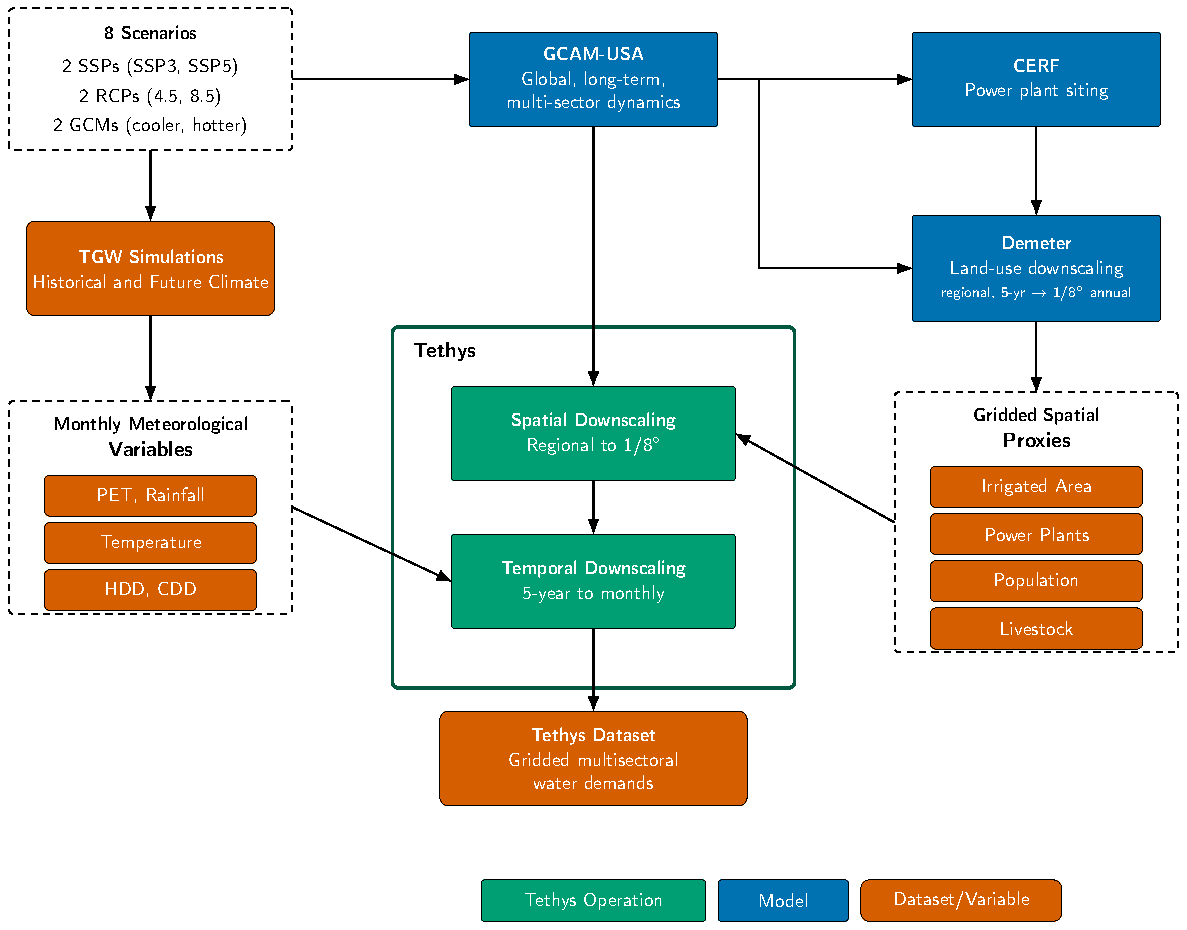
\includegraphics[width=\textwidth]{flow-chart.pdf}
\caption{Workflow for producing the Tethys CONUS multi-sector water-demand dataset for eight scenarios (Table~\ref{tab:scenarios}). Each scenario drives GCAM-USA (regional sectoral demands at the state/basin scale) and TGW-WRF dynamical-downscaling simulations. Tethys (thick outline) carries out the two downscaling operations: spatial downscaling from regional aggregate demands to the 1/8$^{\circ}$ CONUS grid, and temporal downscaling of GCAM-USA outputs to monthly resolution. Spatial downscaling uses gridded proxies derived from Demeter\cite{Vernon-2018} (land use), CERF\cite{Zhao2024,Mongird2025CERF} (projected power-plant siting), Jones and O'Neill\cite{Jones_2016} (population), and GLW~3\cite{Gilbert2018} (livestock). Temporal downscaling uses monthly meteorological variables including potential evapotranspiration (PET), precipitation, mean temperature, heating degree days (HDD), cooling degree days (CDD), and growing-season index (GSI), derived from TGW-WRF\cite{Jones2023TGW}.}
\label{fig:schematic}
\end{figure}

\subsection*{Scenarios}

The dataset spans one historical period (1980--2019) and eight future scenarios (2020--2100), constructed jointly with the IM3/GCIMS framework\cite{Zhao2024,Mongird2025CERF}. The future scenarios include three dimensions: emissions constraints (rcp45 = moderate constraints, rcp85 = no constraints), GCM-temperature sensitivity over CONUS (cooler vs.\ hotter CMIP6 model groups), and Shared Socioeconomic Pathway (SSP3 = low population/economic growth, SSP5 = high growth). Following the IM3/GCIMS convention\cite{Zhao2024,Mongird2025CERF}, we use the acronym ``rcp'' for brevity in scenario names, although the underlying perturbed-thermodynamics simulations are derived from CMIP6, not CMIP5\cite{Mongird2025CERF}. The eight scenario directory names in the dataset (e.g., \texttt{rcp45cooler\_ssp3}) appear in Table~\ref{tab:scenarios} and the inter-scenario behavior of CONUS demand is shown in Figure~\ref{fig:scenarios}.

\subsection*{Meteorological forcing (TGW-WRF)}

The historical and projected meteorological data is from perturbed thermodynamics experiments \cite{Jones2023TGW} (\href{https://tgw-data.msdlive.org/}{https://tgw-data.msdlive.org/}) which provides hourly atmospheric variables at 1/8$^{\circ}$ over CONUS, dynamically downscaled with WRF from a 30-km ERA5 historical baseline (1980--2019) and from CMIP6-derived monthly thermodynamic perturbations (2020--2100). The TGW approach replays historical weather sequences with added thermodynamic signals, retaining the synoptic structure of observed weather while shifting its mean state to match each future scenario. For each TGW scenario we compute daily potential evapotranspiration (PET), precipitation ($P$), mean temperature, heating degree days (HDD), cooling degree days (CDD), and a growing-season index (GSI). These are aggregated to monthly totals or means and reprojected to the Tethys 1/8$^{\circ}$ CONUS grid.

The monthly water deficit used in irrigation temporal downscaling is $\Delta_m = \max\!\big(\text{PET}_m - P_m,\, 0\big)$. The monthly GSI is derived from a simplified version of Jolly et al.\cite{Jolly_2005}, retaining the daily minimum-temperature ($iT_{\min}$) and daylength photoperiod indicators ($iPhoto$) but omitting the vapour-pressure-deficit term. For each day $d$,
\begin{equation}
iT_{\min,d}(T_{\min,d}) = \min\!\left(\max\!\left(\frac{T_{\min,d}+2}{7},\,0\right),\,1\right), \qquad
iPhoto_d(L_d) = \min\!\left(\max\!\left(L_d - 10,\,0\right),\,1\right),
\label{eq:gsi-components}
\end{equation}
where $T_{\min,d}$ is the daily minimum air temperature (\textdegree C) and $L_d$ is the daylength (hours). Monthly GSI is the daily-mean product over month $m$,
\begin{equation}
GSI_m = \big\langle iT_{\min,d} \cdot iPhoto_d \big\rangle_{d \in m}.
\label{eq:gsi-monthly}
\end{equation}
Preprocessing code is archived in the integration meta-repository (see Code availability).

\subsection*{Integrated regional water demand projections (GCAM-USA)}

Region-scale water-demand inputs come from the Global Change Analysis Model (GCAM-USA version)\cite{Zhao_gcamusa_water,Zhao2024,Calvin2019GCAM,Binsted_2022}. GCAM is a market-equilibrium integrated assessment model that allocates supply and demand across coupled energy, water, land, and economic sectors under scenario-specific assumptions on population, productivity, technology, and policy. GCAM-USA resolves U.S.\ electricity generation, manufacturing, and municipal demands at the state level and crop-level irrigation demands at state/basin intersections, at 5-year intervals. 5-year demands are linearally interpolated to annual demands before temporal downscaling is applied. Each of the eight runs corresponds to one scenario; we refer readers to Mongird et al.\cite{Mongird2025CERF} for the full energy-water-land coupling description and limit ourselves here to how the GCAM-USA outputs feed the Tethys workflow shown in Figure~\ref{fig:schematic}.

\subsection*{Power-plant siting projections (CERF)}

Future thermoelectric capacity is sited at $\approx$1-km resolution by the Capacity Expansion Regional Feasibility (CERF) model\cite{Vernon2021,Mongird2025CERF}, which places projected plants based on siting feasibility (exclusion layers, transmission proximity, cooling-water access) and locational economics, conditional on the GCAM-USA state-level capacity trajectory for each scenario. Plants represent thermoelectric generation (coal, natural gas, oil, nuclear, biomass, geothermal, concentrated solar thermal), excluding hydropower. CERF-sited plants are aggregated to 1/8$^{\circ}$ grid cells, and the cell-level installed capacity (MW) serves as the spatial proxy for thermoelectric demand. For the historical period we substitute the 2015 plant inventory from the Global Power Plant Database v1.3 (GPPD), augmented with the IM3 experiment B CONUS plant inventory, in place of CERF projections; both feed the same spatial-downscaling step at the cell.

\subsection*{Land-use projections (Demeter)}

Spatially explicit, scenario-consistent annual per-crop irrigated-area maps at 1/8$^{\circ}$ come from Demeter\cite{Vernon-2018}, a land-use spatial disaggregation model that reconciles a high-resolution land-use baseline with GCAM regional boundary conditions using transition-priority rules that distinguish intensification (increase of a land type within a cell) from extensification (spread from an adjacent cell). For irrigation, Demeter outputs cover the 13 crop classes that GCAM-USA reports (Corn, Wheat, Rice, RootTuber, OilCrop, SugarCrop, OtherGrain, FiberCrop, FodderGrass, FodderHerb, biomass, MiscCrop, PalmFruit). The per-crop irrigated-area fields serve as the spatial proxy for irrigation in the Tethys spatial-downscaling step (see following section for details).

\subsection*{Spatial downscaling}

We assume that the location of demand within a region follows a gridded proxy appropriate to the sector. For any sector with total demand $D_{\mathrm{region}}$ and proxy field $\pi_{\mathrm{cell}}$,
\begin{equation}
D_{\mathrm{cell}} = D_{\mathrm{region}} \times \frac{\pi_{\mathrm{cell}}}{\sum_{c \in \mathrm{region}} \pi_{c}}.
\label{eq:spatial}
\end{equation}
For irrigation, the proxy is per-crop irrigated area from Demeter (described above). For thermoelectric, the proxy is CERF-sited installed capacity (described above). For municipal demand, we use the scenario-consistent gridded population at 10-year intervals from Jones and O'Neill\cite{Jones_2016}, linearly interpolating between bracketing decadal maps, with state-level GCAM-USA municipal demand allocated to cells in proportion to projected population. For livestock, the proxy is the GLW~3 gridded head-count map\cite{Gilbert2018} at 1/12$^{\circ}$ for reference year 2010, re-gridded to 1/8$^{\circ}$ using weighted area-overlap allocation and held fixed across all years and scenarios; livestock is \textasciitilde2\% of CONUS demand, so the static-distribution assumption has limited overall impact (see Limitations). The mapping from GCAM livestock sectors to GLW animals follows Table~\ref{tab:livestock}. For manufacturing and mining, we use population as the spatial proxy, following prior Tethys work\cite{Khan2023}.

\begin{table}[ht]
\centering
\begin{tabular}{ll}
\toprule
\textbf{GCAM livestock sector} & \textbf{GLW proxy animal(s)} \\
\midrule
Beef      & Buffalo + Cattle \\
Dairy     & Buffalo + Cattle \\
Pork      & Pig \\
Poultry   & Chicken + Duck \\
SheepGoat & Sheep + Goat \\
\bottomrule
\end{tabular}
\caption{Mapping from GCAM livestock sectors to animal species in the GLW~3 dataset.}
\label{tab:livestock}
\end{table}

\subsection*{Temporal downscaling}

GCAM-USA operates at 5-year steps. We linearly interpolate spatially-downscaled outputs to annual resolution and then distribute the annual demand at each cell into 12 monthly values using sector-specific formulas. For livestock, manufacturing, and mining we hold monthly demand uniform at $1/12$ of the annual total; irrigation, electricity, and domestic follow climate-driven formulations described next.

\subsubsection*{Irrigation}

For each cell and year, we compute a monthly weight field from the growing-season index $GSI_m$ (Eq.~\ref{eq:gsi-monthly}), the monthly deficit $\Delta_m$, and month length $N_m$ (in days):
\begin{equation}
\tilde{w}_m = \frac{\Delta_m \, GSI_m}{N_m}\quad, \qquad w_m = \frac{\tilde{w}_m}{\sum_{k=1}^{12}\tilde{w}_k},
\label{eq:irr-weights}
\end{equation}
so $\sum_m w_m = 1$ and monthly irrigation demand is $D_{Irrigation,m} = w_m \, D_{Irrigation,\mathrm{year}}$. Equation~(\ref{eq:irr-weights}) combines deficit and growing season approachs of Moore et al.\cite{Moore_2015} and Roy et al.\cite{Roy_2005}. Using this approach, water demand concentrates in months that are simultaneously water-limited ($\Delta_m > 0$) and vegetatively active ($GSI_m > 0$). The weights are computed per-cell and differ across years.

\subsubsection*{Electricity}

We distribute monthly electricity water demand by splitting annual use into heating, cooling, and other shares, each weighted by an HDD/CDD-driven monthly profile. Region-level shares of annual electricity consumption for heating $p_{\mathrm{heat}}$, cooling $p_{\mathrm{cool}}$, and other $p_{\mathrm{other}}$ come from GCAM-USA. At each cell we define annual sums $H_y = \sum_m \text{HDD}_m$ and $C_y = \sum_m \text{CDD}_m$ and monthly distribution fields $\hat{h}_m$ and $\hat{c}_m$ with
\begin{equation}
(\hat{h}_m,\,\hat{c}_m) =
\begin{cases}
\big(\text{HDD}_m / H_y,\ \text{CDD}_m / C_y\big)      & H_y \ge 650 \text{ and } C_y \ge 450 \\[2pt]
\big(\text{HDD}_m / H_y,\ \text{HDD}_m / H_y\big)      & H_y \ge 650 \text{ and } C_y < 450 \\[2pt]
\big(\text{CDD}_m / C_y,\ \text{CDD}_m / C_y\big)      & H_y < 650 \text{ and } C_y \ge 450 \\[2pt]
(\hat{o},\ \hat{o})                                          & H_y < 650 \text{ and } C_y < 450,
\end{cases}
\label{eq:elec-cases}
\end{equation}
with $\hat{o} = 1/12$. 
The first case applies to cells with both a meaningful heating season (annual HDD $\ge 650$) and a meaningful cooling season (annual CDD $\ge 450$). The second and third cases collapse onto whichever signal is non-trivial, preventing division by near-zero annual sums in climates dominated by one extreme. The fourth case reverts to a uniform distribution where neither threshold is exceeded. The threshold convention follows Huang et al.\cite{Huang2018}. Once $\hat{h}_m$ and $\hat{c}_m$ are computed, monthly demand is then downscaled from annual ($D_{Electricity,m}$) demand ($D_{Electricity,\mathrm{year}}$)
\begin{equation}
D_{Electricity,m} = D_{Electricity,\mathrm{year}} \times \big(p_{\mathrm{heat}}\,\hat{h}_m + p_{\mathrm{cool}}\,\hat{c}_m + p_{\mathrm{other}}\,\hat{o}\big).
\label{eq:elec-demand}
\end{equation}


\subsubsection*{Domestic}

For the Municipal (a.k.a. domestic or public-supply) sector we use the temperature-anomaly formula of Wada et al.\cite{Wada2011}:
\begin{equation}
D_{Municipal,m} = \frac{D_{Municipal,\mathrm{year}}}{12} \times \left(\frac{T_m - \bar{T}}{T_{\max} - T_{\min}}\,R + 1\right),
\label{eq:dom-monthly}
\end{equation}
where $T_m$ is the monthly mean temperature at the cell, $\bar{T}$ is the annual mean temperature, $T_{\max}$ and $T_{\min}$ are the annual extremes, and $R$ is a region-scale amplitude coefficient drawn from a static regional map; higher $R$ implies stronger seasonal amplification. We clip negative values to zero so that $D_{Municipal,m} \ge 0$ in every cell. Note that USGS refers to the municipal sector as Public Supply which can encompass Domestic and Industrial water use that is supplied by publicly owned water rights.

\subsection*{Groundwater vs.\ surface water source-share post-processing}

GCAM-USA (Superwell) solves for the share of each basin's withdrawals met from surface versus groundwater supply using by cost-based allocation. Mapping that basin-scale split onto the 1/8$^{\circ}$ grid requires two steps. First, we apply the basin-level share uniformly to all end-use sectors in the basin, except that thermoelectric demand is assumed to use surface water only and the remaining sectoral shares are renormalized accordingly. Second, we anchor the historical spatial pattern of the gw/sw split to USGS data by rescaling each cell's GCAM share against its USGS-2020 value while preserving the spatial pattern of a static USGS baseline derived from the 2009-2020 mean gw/sw share distribution\cite{Stets2025USGS}. Let $s^{\mathrm{GCAM}}_{c,y}$ denote the GCAM-derived renewable share at cell $c$ in year $y$, and $s^{\mathrm{USGS}}_c$ the static USGS-derived baseline share at cell $c$. For the subset of cells $\mathcal{M}$ for which both $s^{\mathrm{GCAM}}_{c,\,2015}>0$ and $s^{\mathrm{USGS}}_c$ is available, the adjusted share is
\begin{equation}
s^{\mathrm{adj}}_{c,y} =
\begin{cases}
\displaystyle \min\!\left(1,\; s^{\mathrm{USGS}}_c \times \frac{s^{\mathrm{GCAM}}_{c,y}}{s^{\mathrm{GCAM}}_{c,\,2015}}\right) & c \in \mathcal{M} \\[10pt]
s^{\mathrm{GCAM}}_{c,y}                                                                                        & c \notin \mathcal{M}.
\end{cases}
\label{eq:source-shares}
\end{equation}
The $\min(\cdot,1)$ clip prevents amplifications when the 2015 GCAM baseline is small. In groundwater-dominated regions the clip can mask trajectory increases, but it preserves the physical bound that a share cannot exceed one. This approach is a compromise that captures GCAMs global dynamics and more closely mimics the USGS split which is computed based on the number of surface water and groundwater intakes in each HUC12 region \cite{Stets2025USGS}.

\subsection*{Modular earth system model coupling}

The dataset combines simulation outputs produced, in some cases, by independent teams that use consistent scenario assumptions.  GCAM-USA is run for each scenario, Demeter is run with the corresponding GCAM-USA scenario to produce per-crop irrigated-area maps; CERF sites power plants using GCAM-USA state-level capacity trajectories; the Jones and O'Neill population maps are used based on the corresponding SSP scenario; and the TGW-WRF climate sample is drawn from a fixed ensemble conditioned on the RCP. We do not perfectly co-calibrate these inputs, which would be prohibitively expensive computationally; instead, we document the specific versions used (see Code availability) and treat the resulting record as scenario-plausible but not a fully coupled  Earth-system simulation. This modular ``frankenstein'' coupling is an established compromise in multi-sector dynamics modeling\cite{Khan2023} and is appropriate for a dataset intended to support sensitivity and adaptation studies, not causal attribution. The combined modeling chain: $\to$ TGW-WRF forcing $\to$ GCAM-USA $\to$ spatial downscaling with proxies $\to$ temporal downscaling with weather dependent weights $\to$ USGS-anchored gw/sw split --- produces the 1/8$^{\circ}$ monthly gridded record described next.

% -----------------------------------------------------------------------------
\section*{Data Records}

The dataset is permanently archived and openly available on MSD-Live (\url{https://data.msdlive.org/uploads/p4xce-e8822}); the Tethys model source is at \href{https://github.com/JGCRI/tethys}{github.com/JGCRI/tethys}.

Scenario directories (Table~\ref{tab:scenarios}) each contain per-sector netCDF~4 files following the naming convention:\\\texttt{<Sector>\_<demand\_type>[\_monthly].nc}, where \texttt{<Sector>} is one of \{\texttt{Domestic}, \texttt{Electricity}, \texttt{Irrigation}, \texttt{Livestock}, \texttt{Manufacturing}, \texttt{Mining}\}, and \texttt{<demand\_type>} is \texttt{withdrawals} or \texttt{consumption}. The \texttt{\_monthly} suffix marks monthly files; for irrigation, the \texttt{\_with\_losses} suffix marks files that include conveyance losses.

Each scenario directory also contains \texttt{gridded\_runoff\_shares.nc} (per-year, per-cell renewable share $s^{\mathrm{adj}}_{c,y}$ from Eq.~\ref{eq:source-shares}, used to recover the surface/groundwater split of withdrawals) and two YAML configuration files (\texttt{config\_withdrawals.yaml}, \texttt{config\_consumption.yaml}) that record the exact Tethys run configuration used to produce the files. All netCDF file shares the same dimensions \texttt{(year, lat, lon)} (for annual data) or \texttt{(year, lat, lon, month)} (for monthly data) with sector-specific sub-variables; 
%Figure~\ref{fig:data-listing} shows an example CDL listing. 
Table~\ref{tab:scenarios} enumerates the eight scenarios. 

% Need to revise this based on new runs
\begin{table}[!ht]
\centering
\begin{tabular}{lll}
\toprule
\textbf{Scenario directory} & \textbf{Time span} & \textbf{Description} \\
\midrule
\texttt{historical}         & 1980--2019 & Observed-period baseline using historical climate and population. \\
\texttt{rcp45cooler\_ssp3}  & 2020--2100 & Lower-emissions, cooler TGW boundary conditions, SSP3 socioeconomics. \\
\texttt{rcp45cooler\_ssp5}  & 2020--2100 & Lower-emissions, cooler boundary conditions, SSP5 socioeconomics. \\
\texttt{rcp45hotter\_ssp3}  & 2020--2100 & Lower-emissions, hotter boundary conditions, SSP3 socioeconomics. \\
\texttt{rcp45hotter\_ssp5}  & 2020--2100 & Lower-emissions, hotter boundary conditions, SSP5 socioeconomics. \\
\texttt{rcp85cooler\_ssp3}  & 2020--2100 & Higher-emissions, cooler boundary conditions, SSP3 socioeconomics. \\
\texttt{rcp85cooler\_ssp5}  & 2020--2100 & Higher-emissions, cooler boundary conditions, SSP5 socioeconomics. \\
\texttt{rcp85hotter\_ssp3}  & 2020--2100 & Higher-emissions, hotter boundary conditions, SSP3 socioeconomics. \\
\texttt{rcp85hotter\_ssp5}  & 2020--2100 & Higher-emissions, hotter boundary conditions, SSP5 socioeconomics. \\
\bottomrule
\end{tabular}
\caption{Scenario directories in the published dataset. Each directory contains per-sector withdrawal and consumption netCDFs, a gridded runoff-share file, and the two Tethys YAML configurations used to generate them.}
\label{tab:scenarios}
\end{table}

%\begin{figure}[ht]
%\centering
%\begin{verbatim}
%netcdf Livestock_withdrawals_monthly {
%dimensions:
%    year = 46 ;
%    lat = 224 ;
%    lon = 464 ;
%    month = 12 ;
%variables:
%    float Beef(year, lat, lon, month) ;
%    float Dairy(year, lat, lon, month) ;
%    float Pork(year, lat, lon, month) ;
%    float Poultry(year, lat, lon, month) ;
%    float SheepGoat(year, lat, lon, month) ;
%    double lat(lat) ;
%    double lon(lon) ;
%    int64 year(year) ;
%    int64 month(month) ;
%    int64 spatial_ref ;
%}
%\end{verbatim}
%\caption{CDL excerpt of a monthly livestock-withdrawals netCDF. Other sectors share the same \texttt{(year, lat, lon [, month])} layout with sector-specific sub-variables.}
%\label{fig:data-listing}
%\end{figure}

% -----------------------------------------------------------------------------
\section*{Technical Validation}

We validate the downscaled dataset against the latest USGS dataset\cite{Stets2025USGS}, refreshed in January~2025, for three sectors that together account for over 90\% of CONUS water demand: irrigation, thermoelectric, and domestic (public supply)\cite{skinnerWaterWithdrawalConsumption2025}. The goal is to establish that the downscaled record reproduces the dominant features of spatial and temporal demand and quantified bias where it departs, recognizing that both USGS and Tethys are model-derived datasets with distinct modeling assumptions with limited direct observations. The USGS data is provided at the HUC12 scale and was mapped to the Tethys 1/8$^{\circ}$ grid using an area weighted aggregation approach. Livestock, Manufacturing, and Mining are not validated against USGS at HUC6 because they rely on static or population-proxy spatial allocation (see Limitations).


\begin{table}[ht]
\centering
\begin{tabular}{lcccccc}
\toprule
\textbf{Sector} & \textbf{Pearson r} & \textbf{MBE (\%)} & \textbf{MAPD (\%)} \\
\midrule
Domestic     & 0.95 & $+7$  & 37 \\
Electricity  & 0.73 & $-2$  & 86 \\
Irrigation   & 0.89 & $-2$  & 79 \\
\bottomrule
\end{tabular}
\caption{Validation metrics for withdrawals in the three sectors that together account for over 90\% of CONUS water demand, against USGS 2025 water demand data (2010--2020) at the HUC6 scale ($n=329$ HUC6 basins for Domestic, $n=230$ for Electricity, $n=297$ for Irrigation; differences reflect basins where USGS reports zero use for that sector). Metrics are computed HUC6 means: USGS monthly demand summed to annual at each HUC6 and averaged across reporting years. Domestic USGS values are scaled by 1.12 to align with the public-supply-only definition introduced after 2015~\cite{Stets2025USGS}. Reported metrics include Pearson correlations, Mean Bias (MB), and Median Absolute Percent Difference (MAPD).}
\label{tab:validation-metrics}
\end{table}

\subsection*{CONUS annual totals}

Figure~\ref{fig:annual-total-timeseries} compares CONUS-aggregated annual demand for each of the three sectors and their sum. Tethys reproduces the magnitude of USGS CONUS totals within roughly 10\% at and annual resolution and follows the long-term trend (See Table~\ref{tab:validation-metrics}). Magnitudes differ sharply across sectors, as expected: irrigation dominates consumptive use, while thermoelectric and irrigation withdrawals are of comparable magnitude. The decline in Electricity withdrawals reflects a known trend driven largely by the switch from coal-fired plants to other technologies\cite{skinnerWaterWithdrawalConsumption2025}. The GCAM-USA 5-year time step manifests in Tethys annual irrigation demands as reduced interannual variability relative to USGS. Figure~\ref{fig:annual-total-boxplot} shows the distribution of percent difference between the two datasets across HUC6 regions, further reflecting the dominance of CONUS irrigation water.

\begin{figure}[ht]
\centering

\includegraphics[width=\linewidth]{val1-huc06-usgs-tethys-annual-total.png}
\caption{CONUS annual water use by sector from Tethys (black) and USGS (orange), 2000--2020.}
\label{fig:annual-total-timeseries}
\end{figure}

\begin{figure}[ht]
\centering

\includegraphics[width=\linewidth]{val2-huc06-usgs-tethys-annual-total-pdiff.png}
\caption{Percent difference between Tethys and USGS annual water use across HUC6 regions ($n=329$ basins for Domestic, 230 for Electricity, 297 for Irrigation), by sector and demand type. Boxplot whiskers represent 1.5 times the interquartile range (IQR).}
\label{fig:annual-total-boxplot}
\end{figure}

\subsection*{HUC6 spatial agreement}

Figure~\ref{fig:map-pbias} maps the percent difference in annual average use at the HUC6 scale. Tethys tends to exceed USGS in the Electricity sector, especially in the eastern U.S.~where thermoelectric plants are more highly concentrated. Spatially, the Tethys and USGS datasets most strongly disagree for Irrigation demands (both withdrawals and consumption). Basin-wise correlations (Figure~\ref{fig:huc-correlation}) are relatively strong for annual average data, with Domestic demands having the highest correlation ($r=0.95$), followed by Irrigation ($r=0.89$), and Electricity ($r=0.73$). The points in Figure~\ref{fig:huc-correlation} are also colored by basin area which shows no discernible pattern, indicating that basin area is not a string indicator of the difference between the two datasets

\begin{figure}[ht]
\centering

\includegraphics[width=\linewidth]{val3-huc06-pdiff-usgs-tethys.png}
\caption{Percent difference in annual-average HUC6 water use, Tethys minus USGS, for Domestic, Electricity, and Irrigation sectors.}
\label{fig:map-pbias}
\end{figure}

\begin{figure}[ht]
\centering

\includegraphics[width=\linewidth]{val4-huc06-scatter-usgs-tethys.png}
\caption{HUC6 annual average demand, Tethys versus USGS, by sector and demand type. Pearson correlations: 0.95 (Domestic), 0.73 (Electricity), 0.89 (Irrigation), computed on per-HUC6 means across the USGS reporting years 2010--2020.}
\label{fig:huc-correlation}
\end{figure}

% AI nonsense section -_-
%\subsection*{Bias diagnosis and uncertainty}

%The mean bias (MBE is small  (within $\pm 7\%$ for all three sectors at HUC6, Table~\ref{tab:validation-metrics}), but the residual NRMSE and MedAPE remain large because per-basin biases compensate. The dominant per-basin pattern is a Domestic over-prediction in many basins ($\text{MedAPE} \approx 37\%$, modest aggregate $+7\%$ MBE after the public-supply 1.12 scaling), most likely attributable to the calibration of the Wada\cite{Wada2011} $R$ amplitude coefficient in Eq.~(\ref{eq:dom-monthly}), which was fit to aggregate USGS demand and may not capture the post-2015 public-supply subset, and to a mismatch in the GCAM-USA base-year socioeconomic data relative to USGS 2015 reporting. Electricity has the lowest spatial agreement ($r=0.73$, Table~\ref{tab:validation-metrics}) and the largest within-basin spread (NRMSE $\approx 171\%$, MedAPE $\approx 86\%$): GCAM-USA represents thermoelectric water use at state aggregates that already trail observed plant-by-plant cooling-water reductions over 2010--2015, and the CERF-sited capacity proxy concentrates demand at projected build-out locations rather than at the historical plant locations USGS observes, which produces the basin-by-basin scatter visible in Figure~\ref{fig:annual-total-boxplot}. Irrigation tracks USGS most closely in aggregate ($\text{MBE} \approx -2\%$) but with comparable per-basin spread (NRMSE $\approx 130\%$, MedAPE $\approx 79\%$), driven by the western-basin underweighting visible in Figure~\ref{fig:map-pbias}. Reference USGS estimates themselves carry inherent uncertainties, particularly in the thermoelectric and irrigation sectors, as documented in recent reanalyses\cite{Harris2025, Stets2025USGS}.

\subsection*{Seasonal cycle}

Figure~\ref{fig:monthly} compares the mean monthly demands for each HUC6 basin. Irrigation and Electricity withdrawals reproduce the seasonal shape observed by USGS closely. Electricity consumption shows a consistent low offset in non-summer months, likely from the GCAM-USA representation of non-cooling electricity water use. Domestic shows the small positive aggregate bias seen in the annual MBE (Table~\ref{tab:validation-metrics}, $+7\%$); the seasonal amplitude tracks USGS, with month-to-month departures driven by the temperature-anomaly term in Eq.~(\ref{eq:dom-monthly}) interacting with the static $R$ regional map, which was calibrated to aggregate USGS demand rather than to the post-2015 public-supply subset.

\begin{figure}[ht]
\centering

\includegraphics[width=\linewidth]{val5-huc06-usgs-tethys-monthly-total.png}
\caption{Mean monthly CONUS water use by sector, Tethys (black) and USGS (orange), averaged over 2000--2020.}
\label{fig:monthly}
\end{figure}

\subsection*{Inter-scenario consistency}

Figure~\ref{fig:scenarios} shows CONUS annual demand across the historical and eight future scenarios for the three largest sectors and their sum. We connect each future scenario to the historical line at 2019 so the visual hand-off does not introduce a spurious 2015--2020 gap; the small offset that remains at the historical-to-future junction reflects the switch from the ERA5-based reanalysis run to the TGW-driven future simulations, which replay the historical weather sequence with added thermodynamic warming, and is a known artifact of the modular forcing chain rather than a physical change. The scenario spread exhibits the expected signature of each input: strong SSP-driven divergence in Domestic (SSP5 rising with population, SSP3 declining), large inter-scenario variability in Irrigation driven by RCP, and a monotone decline in Electricity across all futures that reflects the GCAM-USA projection of declining thermoelectric water use under continued fleet turnover. Within the future period the scenarios evolve smoothly with no further artifacts, supporting use of the inter-scenario contrasts.

\begin{figure}[ht]
\centering
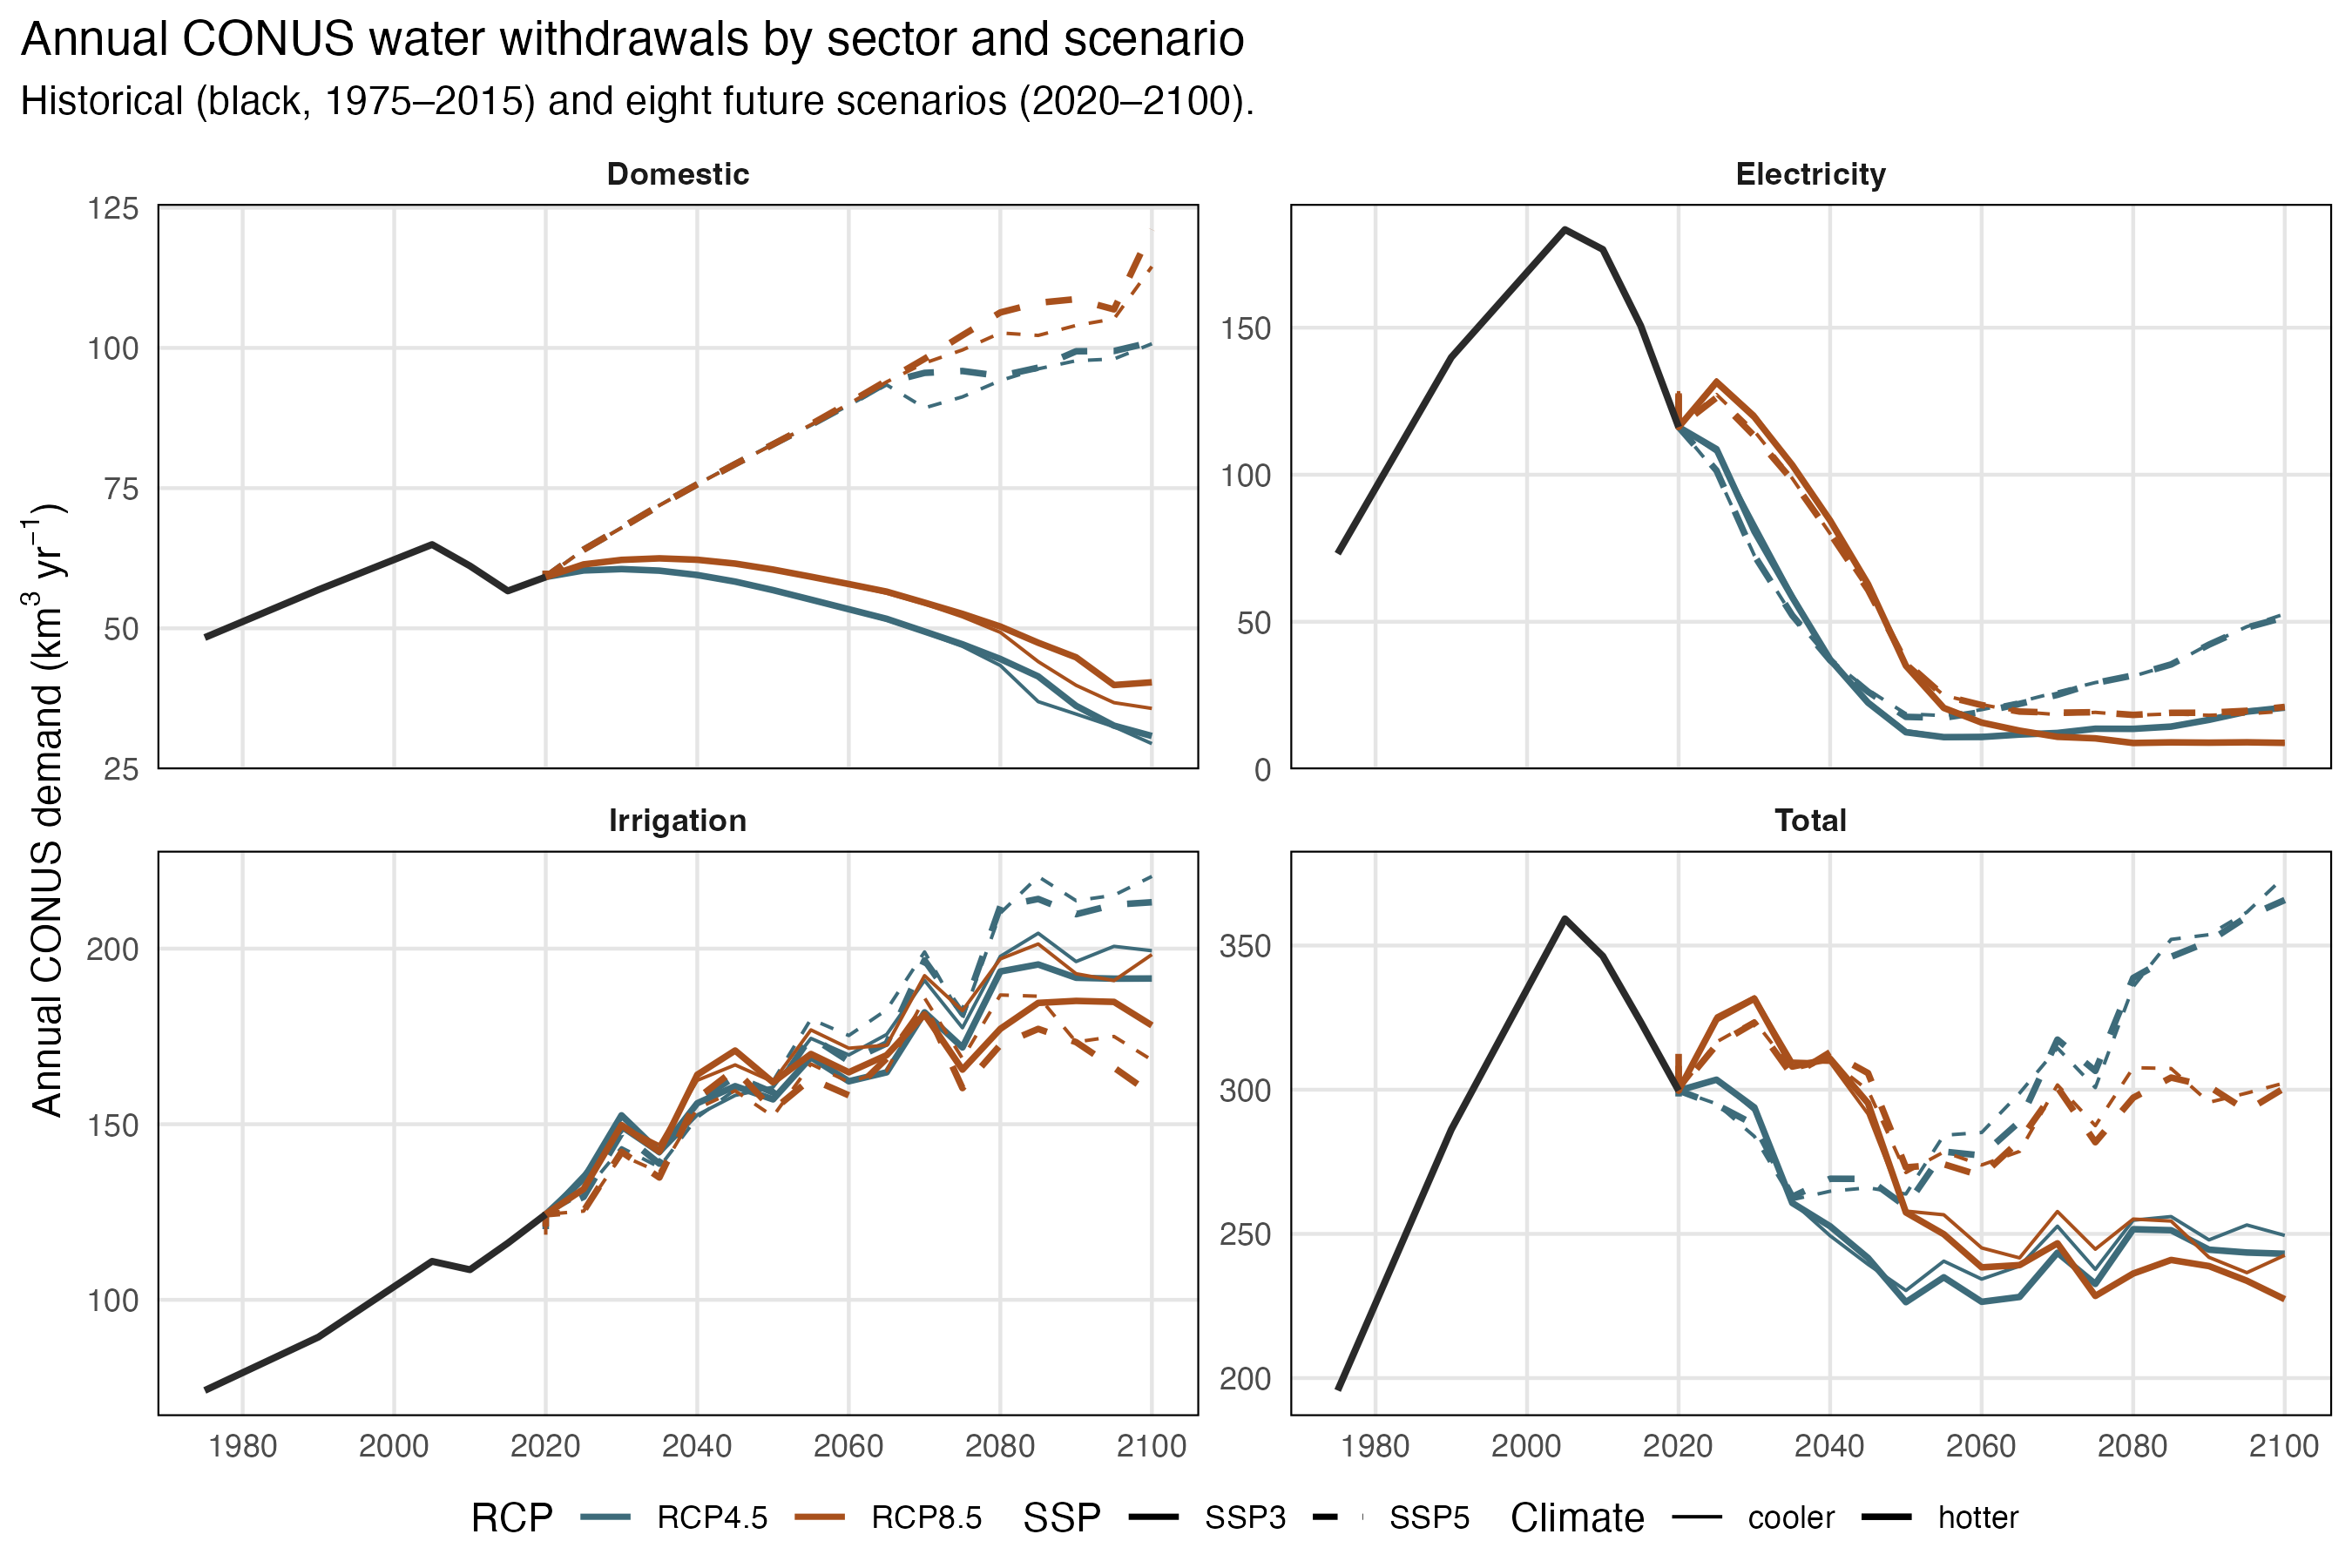
\includegraphics[width=\linewidth]{usage2-projections-annual-conus-timeseries.png}
\caption{Annual CONUS water withdrawals by sector and scenario. The historical simulation (black, 1975--2019) is connected to each of the eight future scenarios (2020--2100) at 2019 so the hand-off is continuous in the visual; future scenarios vary by RCP (color), climate-model sample (line width), and SSP (line style). Each panel uses an independent $y$-axis.}
\label{fig:scenarios}
\end{figure}

\subsection*{HDD/CDD threshold sensitivity (Eq.~\ref{eq:elec-cases})}

The piecewise definition in Eq.~(\ref{eq:elec-cases}) describes four cases defined by specific HDD and CDD thresholds $H_{\mathrm{thr}}=650$ and $C_{\mathrm{thr}}=450$ from Huang et al.\cite{Huang2018}. We tested the sensitivity of the thresholds and the resulting monthly weights by perturbing the thresholds by $\pm 50\%$, holding the GCAM-USA shares $(p_{\mathrm{heat}}, p_{\mathrm{cool}}, p_{\mathrm{other}})$ fixed at $(0.20, 0.40, 0.40)$. Under the default thresholds, 32\% of CONUS cell-years fall in case~1 (both heating and cooling seasons present), 46\% in case~2 (heating only), 19\% in case~3 (cooling only), and 3\% in case~4 (uniform). Halving the thresholds to $(325, 225)$ moves the partition toward case~1 (49\%, 35\%, 16\%, 0\%); raising them by 50\% to $(975, 675)$ moves it toward case~2 (20\%, 54\%, 22\%, 5\%). The weights shifts the weights up by at most $\approx 1.8$ \% points and down by $\approx 1.1$~\% Figure~\ref{fig:eq5-sensitivity}. This indicated that the monthly Electricity weights are reasonably insensitive to the choice of HDD and CDD thresholds. 

\begin{figure}[ht]
\centering

\includegraphics[width=\linewidth]{eq5-hdd-cdd-sensitivity.png}
\caption{Sensitivity of Eq.~(\ref{eq:elec-cases}) to the HDD/CDD thresholds, computed over CONUS for the historical reference decade (2010--2019). (a) Stacked partition fractions of cell-years into the four cases under the default $(650, 450)$ thresholds and $\pm 50\%$ perturbations. (b) CONUS-mean Electricity monthly weight profile resulting from each threshold pair, holding the GCAM-USA $(p_{\mathrm{heat}}, p_{\mathrm{cool}}, p_{\mathrm{other}})$ shares fixed at $(0.20, 0.40, 0.40)$ to isolate the sensitivity to the case partition.}
\label{fig:eq5-sensitivity}
\end{figure}

\subsection*{Limitations}

Several known limitations should inform reuse of the dataset, grouped here into spatial-stationarity caveats and methodological caveats. \emph{Livestock spatial stationarity:} the GLW~3 livestock distribution is held fixed at 2010 across all years and scenarios. Livestock is \textasciitilde2\% of CONUS demand, but within individual basins --- particularly in states with rapidly shifting livestock composition --- this may introduce local bias. \emph{Manufacturing and mining proxy:} using population as the proxy for these two sectors captures average patterns of labor-associated demand but misses site-specific industrial or mining facilities whose water withdrawals can dominate local basin totals.

On the methodological side, the \emph{electricity source-share carve-out} in Eq.~(\ref{eq:source-shares}) assigns thermoelectric demand to surface water only and renormalizes remaining-sector shares; where a thermoelectric plant is served from a local groundwater source (rare but documented), this assumption places the withdrawal on surface water and slightly overstates surface demand elsewhere. \emph{Riparian vs.\ reservoir allocation:} the dataset represents demand at the cell where use occurs, which is not necessarily the cell from which water is withdrawn in reservoir-fed or interbasin-transfer systems; downstream routing and water-management models (e.g., mosartwmpy) handle the supply-side re-allocation. The \emph{simplified GSI} used for irrigation temporal downscaling (Eqs.~\ref{eq:gsi-components}--\ref{eq:gsi-monthly}) drops the vapour-pressure-deficit (VPD) component of the original Jolly et al.\cite{Jolly_2005} formulation; this simplification is consistent with Moore et al.\cite{Moore_2015} but may underweight drought months in humid climates where VPD is the binding constraint. \emph{Conveyance losses:} irrigation files exist with and without conveyance losses applied (\texttt{\_with\_losses} suffix), and users coupling the dataset to hydrologic routing should select the appropriate variant for their application. \emph{GCAM-USA temporal interpolation:} the 5-year GCAM step linearly interpolated to annual resolution suppresses interannual variability and is most visible as smoother trend lines in irrigation, which makes the dataset appropriate for scenario-level and climatological-mean analyses but not for replicating year-to-year demand variability.

% -----------------------------------------------------------------------------
\section*{Usage Notes}

We distribute the dataset as netCDF~4 files. The netCDF files contain year and month dimensions. Each file contains either withdrawals or consumption in km$^3$~yr$^{-1}$. Users convert from the native unit (km$^3$~yr$^{-1}$) to MGD by multiplying by $264{,}172.05124/365$, so $1\text{ km}^3\text{ yr}^{-1} \approx 723.76$~MGD.

The companion integration meta-repository provides HUC-level aggregation utilities that use the \texttt{xagg} library to compute aggregations from the 1/8$^{\circ}$ grid to HUC2, HUC4, HUC6, HUC8, or HUC12 polygons; see the meta-repository README for usage.

The dominant water-use sector at each 1/8$^{\circ}$ cell shown in Figure~\ref{fig:dominant-sector} (front of paper) is one example product that exercises the full multi-sector resolution, additional advances are itemized in the next section.

\section*{Improvements over previous version}

Compared with the prior Tethys global product\cite{Khan2023}, the dataset presented here advances the representation of demand in six specific ways.

\paragraph{GCAM-USA integration.} The prior record used the global GCAM configuration, which disaggregated U.S.~demand from a single national total. This dataset uses GCAM-USA, which resolves U.S.~electricity generation, manufacturing, and municipal demand at the state level and crop irrigation demand at state$\,\times\,$basin intersections. State-level inputs eliminate the artifact of national-average demand being pushed uniformly into states with very different sectoral mixes, and they allow the subsequent spatial downscaling to respect state-level regulatory and policy boundaries.

\paragraph{CERF-based power-plant siting.} Prior gridded electricity demand used population as the spatial proxy, which approximates the location of load rather than the location of cooling demand. This dataset uses explicit power-plant siting from the CERF model\cite{Vernon2021}, which places thermoelectric plants at $\approx$1-km resolution based on siting feasibility (exclusion layers, transmission proximity, cooling-water access) and then aggregates installed capacity to the 1/8$^{\circ}$ grid as the proxy. The result places thermoelectric demand at actual generation sites rather than at population centroids, correcting the historical decoupling of load from generation in regions like the lower Colorado and Tennessee Valley.

\paragraph{SSP-consistent population.} Prior work used a static base-year population map to distribute municipal, manufacturing, and mining demand across all years, including future projections. This dataset uses SSP3 and SSP5 gridded population projections from Jones and O'Neill\cite{Jones_2016}, linearly interpolated from their decadal native resolution to annual values. Scenario-consistent population is essential for the SSP-differentiated futures: SSP3 and SSP5 diverge markedly in U.S.~population growth, and that divergence propagates into the public-supply demand field in a way that a static map cannot represent.

\paragraph{GSI-based irrigation temporal downscaling.} Prior irrigation monthly weights used a simpler temperature-driven scheme. This dataset computes per-cell monthly weights (Eq.~\ref{eq:irr-weights}) from the TGW-WRF monthly deficit and growing-season index, so the monthly distribution of irrigation demand responds to climate-consistent drought and growing-condition signals rather than to a static seasonal template. The monthly irrigation distribution thus varies from year to year and across scenarios, tracking interannual drought variability that a static template cannot reproduce.

\paragraph{USGS-anchored source-share attribution.} Prior work applied GCAM's basin-level renewable vs.\ non-renewable split uniformly across cells within each basin. This dataset uses Eq.~(\ref{eq:source-shares}) to anchor the historical 2015 spatial pattern to USGS baseline observations while preserving the temporal evolution from GCAM. In regions with observable baseline data this reduces bias relative to the GCAM-uniform allocation (see Technical Validation); outside those regions, the GCAM share is preserved.

\paragraph{Resolution refinement.} Spatial resolution is refined from 1/2$^{\circ}$ to 1/8$^{\circ}$, a factor-of-4 improvement per dimension and a factor-of-16 improvement in areal resolution. Combined with the finer proxy data (CERF plants at \textasciitilde1~km, Demeter LULC at 1/8$^{\circ}$, Jones population at 1/8$^{\circ}$), the 1/8$^{\circ}$ grid allows the resulting demand field to represent sub-state variation relevant to river routing, reservoir management, and local planning applications.

Together, these six advances produce a dataset that captures HUC6 spatial pattern (annual correlations of 0.73--0.95) and supports detailed scenario analysis against the refreshed January~2025 USGS water-use record, which includes updated thermoelectric cooling-water estimates\cite{skinnerWaterWithdrawalConsumption2025}. As discussed in Technical Validation, the close per-sector mean-bias agreement (within $\pm 7\%$) masks substantial within-basin spread (NRMSE 68--171\%, MedAPE 37--86\%); downstream users computing per-sector scarcity at individual basins should consult Table~\ref{tab:validation-metrics} and the HUC6 maps rather than rely on aggregate agreement alone.

% -----------------------------------------------------------------------------
\section*{Code and external data availability}

\begin{itemize}
    \item \textbf{Tethys downscaling package}: \url{https://github.com/JGCRI/tethys}
    \item \textbf{Integration meta-repository}: \url{https://github.com/IMMM-SFA/tethys_integration_metarepo} and the input dataset \url{https://doi.org/10.57931/3366010}. See the repository README for instructions on reproducing the dataset and figures in this paper.
    %\item \textbf{Demeter} (land-use downscaling, used to produce per-crop irrigated-area proxies): \url{https://github.com/IMMM-SFA/demeter}\cite{Vernon-2018}.
    %\item \textbf{CERF} (power-plant siting): \url{https://github.com/IMMM-SFA/cerf}\cite{Vernon2021}.
\end{itemize}
The TGW-WRF climate forcing\cite{Jones2023TGW} that drives the Tethys runs is available as external data at \url{https://tgw-data.msdlive.org/}. 

% -----------------------------------------------------------------------------
\section*{Acknowledgments}

This research was supported by the U.S.~Department of Energy, Office of Science, as part of research in MultiSector Dynamics, Earth and Environmental System Modeling Program. We thank the TGW-WRF team for the downscaled climate product, the GCAM-USA team for the scenario simulations, and the USGS water-use program for the reference observations used in validation.

\section*{Author contributions statement}

% TODO: coauthors to fill in per CRediT roles. Illustrative template:
C.B.~Coordinated the downscaling runs, conducted the HUC-scale validation, and drafted this version of the manuscript based on an earlier draft by I.T.
H.N.~Developed and maintained the Tethys model, conducted the runs, and helped with the interpretation of GCAM-USA and Tethys outputs.
T.T.~Extended the Tethys package to support GCAM-USA inputs, developed the first version of the Tethys metarepo, and carried out the initial scenario runs.
I.T.~Wrote initial draft of this manuscript, contributed to the CERF--Tethys integration and power-plant proxy construction.
K.T.~Developed the USGS-anchored source-share attribution as a postprocessing to Tethys and conducted runs.
H.E.~Produced the TGW-WRF preprocessing pipeline for PET, HDD/CDD, and GSI.
K.M.~Developed CERF--Tethys integration and power-plant proxy construction.
N.V.~Contributed to scenario design and interpretation.
N.S.~Project management, scenario design and interpretation.
J.R.~Provided overall project guidance and scientific review.

\section*{Competing interests}

The authors declare no competing interests.

\bibliography{bib/Tethys}

\end{document}
